This introduction is split into three parts, corresponding to the three major themes of the thesis. This chapter exists to provide some background on the methods and techniques used as well an outline of the problems that are to be tackled in the thesis proper.

\section{Statistical Ecology}

Some general remarks about stat ecol perhaps.

%\section{Themes}
%
%Some sort of general intro here.
%
%\bi
%	\item Morphing
%	\item Modifying penalties
%	\item Computational efficiency
%	\item Realistic physical models!!!!!!
%\ei


\section{Some notational conventions}
If necessary!

\section{Generalized Additive Models}

General GAM setup. The is will mostly be taken from \cite{simonbook}, \cite{rwc} and \cite{marraradice2010}.

\bi
\item Splines
\item objective function
\label{GAMobjfcn}
\item penalties
\label{GAMpenalties}
\item bases - TPRS (and maybe P-splines?)
\label{GAMtprs}
\label{GAMtprspenalty}
\item tensor products
\label{GAMtensor}
\item fitting - GCV REML etc
\label{GAMGCV}
% see p. 122 RWC here GCV vs REML -> same MSE but different tradeoffs in Var and Bias
\item other stuff - MSE, EDF etc
\item \texttt{mgcv}
%	\bi
%	\item MSE
%	Mean squared error is... (look at HTF)
%	
%	\begin{equation}
%\text{MSE}(\hat{f}) = \frac{1}{P} \sum_{j=1}^P (\hat{f}(x_j) - z_j)^2,
%\end{equation}
%the mean difference between the model ($\hat{f}$) evaluated at the prediction points ($\{x_j : j=1 \dots P\}$) and the true value of the function ($\{z_j : j=1 \dots P\}$.) This gives the MSE per model, since here many realisations are run, the mean of these over all simulations is taken and the standard error is calculated.
%	\item EDF
%	
%The estimated degrees of freedom gives an measure of the complexity of the model that was fit to the data. The higher the EDF, the more basis functions were used and  the more complex the model.  Since the models used here are penalised, it is the penalty term that controls the overall ``wigglyness'' of the spline and hence the EDF. Although the basis dimension is set in the model, this is just an upper bound, the smoothing penalty suppresses parts of the model. Therefore basis dimension is not a major concern provided that it is not set too low (\cite{simonbook}, p. 161.) 
%
%	\ei
\ei

\section{Finite area smoothing}

\subsection{Overview of finite area smoothing}

Splines are a popular way of performing spatial smoothing in two dimensions. In this context, they are often used to fit smooth functions over a geographical region. A typical application of this is in ecological modelling; a response (be it simply the presence of individuals in a population or concentration of a chemical) is modelled as a function of its spatial coordinates. The estimated function can then be used to perform inference on the population, whether that be an abundance estimate, density map or a more sophisticated inferential goal. Finite area smoothing simply specifies that the domain over which this smoothing takes place is bounded.

When the geographical region has a \emph{complex boundary}, features from one part of the domain can unduly influence other parts. Considering the boundary as a polygon, a complex boundary is a non-convex polygon, in particular when the non-convexity is relatively extreme. Often this consists of having some peninsula-like feature(s) in the domain with notably different observation values on either side of the feature. Given that there is some scientific motivation as to why those parts of the domain should not affect each other, features such as peninsulae give rise to a phenomenon known as \emph{leakage}.

Leakage occurs when a smoother inappropriately links two pats of a domain (\cite{soap}). The phenomenon is problematic since it causes the fitted surface to be mis-estimated; this can then lead to incorrect inference (eg. biased abundance estimates), which is clearly not desirable. Leakage can be seen in \fig{leakage} where the high values in the upper half of the domain leak across the gap to the lower values below and vice versa.

% leakage example 
\begin{figure}
\centering
% trim order l b r t
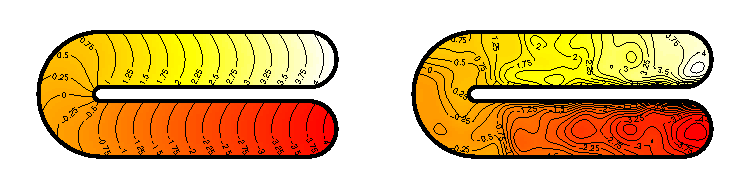
\includegraphics{intro/figs/ramsay-leak.pdf}\\
\caption{An example of leakage. A thin plate regression spline was fit to data sampled from the function on the left, here the model smooths across the gap in the middle of the domain (right.)}
\label{leakage}
\end{figure}

The problem of leakage arises because of the way in which the smoother defines how near objects are to one another. Most smoothing techniques use the Euclidean metric to measure the distance between data. Clearly though, this approach is a flawed: biological populations do not conform to Euclidean geometry in their movement patterns and hence their observed positions will reflect this. Just as whales no not uniformly distribute themselves across sea and glacier, fish do not lay their eggs on land. Natural and man-made barriers carve up the landscape (and seascape), partitioning biological populations; our models should take this into account.

The distribution of the population may be smooth, just not necessarily over $\mathbb{R}^2$ (\cite{wangranalli}). Instead the structure of the domain that is under investigation must be modelled (implicitly or explicitly) for the correct inference to be drawn.

\subsection{Ramsay's horseshoe function as a benchmark for finite area smoothing}

\label{ramsayfunc}

\cite{ramsay} proposes a function which can be used to benchmark new approaches to 2-dimensional smoothing. The function takes the form of a horseshoe shape which is flat across the domain has a gradient along the domain's major axis. This can be seen in \fig{orig-fs}. \cite{soap} modifies the test function by adding curvature across the minor axis of the shape. This was added in order to avoid the horseshoe function lying in the nullspace of their model's penalty, making the problem trivial. It is the second shape that will be used for simulations here and shall be referred to as the \emph{Ramsay horseshoe} throughout; it is shown in \fig{leakage}.

% original horseshoe from Ramsay's paper
\begin{figure}
\centering
% trim order l b r t
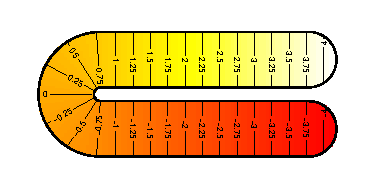
\includegraphics{intro/figs/orig-fs.pdf}\\
\caption{The horseshoe function as it appeared in \cite{ramsay}.}
\label{orig-fs}
\end{figure}

The test function highlights leakage well. As mentioned above, when the smoothing problem is specified in terms of Euclidean distance, the model takes the distance between the points in the two arms of the horseshoe as the distance over the gap in-between them, rather than the distance along the major axis of the shape. This causes the high function values from one side to contaminate the other side (and the low to contaminate the high.) It is easy to see that this causes the smooth to be an inappropriate model.
		
\subsection{Previous approaches to leakage}

The cause of leakage can be characterised in two ways: either the smooth does not respect the boundary of the domain, or the smooth does not take into account the geometry of the domain (in particular with regard to the distance between points within the domain). Previous work in this area has been to combat leakage along these two lines. Work of \cite{ramsay} and \cite{soap} both use a partial differential equation (PDE) boundary condition approach to try to prevent leakage, where as \cite{wangranalli} and \cite{eilerstalk}  attempt to approximate the intrinsic structure of the domain while not treating the boundary as something special in the basis setup. These four main works may be summarised as follows:

\begin{enumerate}
\item \cite{ramsay} proposes finite element $L$-splines (FELSPLINEs). The $L$-spline replaces the usual penalty term (see \secref{GAMpenalties}) with:
\be
\int_\Omega (L_p f)^2 \text{d}\Omega,
\ee
where $\Omega$ is the domain in question and $L_p$ is a roughness operator defined as:
\be
L_p=\Delta^p+c_{p-1}\Delta^{p-1}+\dots+c_1\Delta+c_0I.
\ee
Here $I$ is the identity operator, the $\{c_0,\dots, c_p\}$ are constants and the $\Delta$ is the Laplacian ($\Delta f = f_{xx}+f_{yy}$ in the usual notation). Although any differential operator could, in principle, be used for $L_p$, the Laplacian gives rise to a set of polynomials which are rotation and translation invariant which is clearly sensible given the objective function solution should not depend on the coordinate system used.

In order to find the minimiser of the objective function, Ramsay takes a finite element approach. First he triangulates the domain, then he constructs a set of bivariate quadratic polynomial basis functions over each triangle, specifying that there be continuity over the edges of the triangles. By taking the FELSPLINE objective function and transforming it into a variational form (in the same way as a PDE is), the approximation to the minimiser of the objective function is found. 

Since the triangulation and hence the penalty of the FELSPLINE is only calculated over the domain, and the continuity is specified over neighbouring cells, the method prevents leakage. However, although FELSPLINE does not exhibit leakage on the original horseshoe (as in \fig{orig-fs}), in practice the model makes unrealistic physical assumptions. The boundary conditions of FELSPLINE specify that the gradient is zero, along normals to the boundary. This is not always physically realistic. \cite{soap} show that by using a different response function for the horseshoe shape, the FELSPLINE performance begins to falter.

FELSPLINE does not offer a realistic physical model and is therefore not a viable solution to the finite area smoothing problem in general.

\item \cite{wangranalli} adopt a ``within-area distance'' formulation for thin plate splines. They choose to use the geodesic distance between two points, that being the shortest path within the domain. This gives a definition of how near objects are in the domain. This is then used as the distance in the radial basis functions of a \tprs, rather than using the usual Euclidean distance (see \secref{GAMtprs}).

Wang and Ranalli first create a weighted, undirected graph ($G$, say) with a data point at each vertex and the distance between each pair of vertices as the weights on the edges. They then take the restricted graph of $G$, $G_k$, in which each vertex is only connected to its $k$ nearest neighbours. With this new, restricted graph the geodesic distances between each pair of vertices can be calculated using Floyd's algorithm (\cite{Floyd}).

As the authors point out, the quality of the approximation is dependent on the size of the data set and its density. At low densities the estimated geodesic distance will tend towards the Euclidean, at high densities the approximation tends, asymptotically toward the true geodesic distance (\cite{bernstein}). Even if  dense enough data were available, the method will be rather slow since Floyd's algorithm is cubic in the number of vertices (the size of the data set). Finally, although the $k$-nearest neighbours algorithm used is not specified in the paper, in general such procedures are computationally expensive, adding another source of impedance to the technique.

Taking these points into account, Wang and Ranalli's approach appears cumbersome, slow and dependent on dense data.

\item The soap film smoother (\cite{soap}) uses a rather simple physical model to prevent leakage from occurring. First, consider the domain boundary to be made of wire, then dip this wire into a bucket of soapy water, you will then have (provided it doesn't pop(!)) a soap film in the shape of your boundary. Now consider the wire to lie in the $x-y$ plane and the height of the soap film at a given point to be the functional value of the model. This film is then distorted smoothly by moving it toward the data, while minimising the surface tension in the film. The domain ($\Omega$) is bounded by some polygon with boundary conditions that are either known or estimated by a cyclic spline.

Mathematically, the soap film smoother is constructed by first specifying a set of functions $\rho_k(x,y)$, which are each solutions to the Laplace equation in two dimensions:
\be
\frac{\partial^2\rho}{\partial x^2} + \frac{\partial^2\rho}{\partial y^2} = 0
\ee
except at one of the knots ($x^*_k,y^*_k$). Then, solving Poisson's equation in 2-dimensions:
\be
\frac{\partial^2 g_k}{\partial x^2} + \frac{\partial^2 g_k}{\partial y^2} = \rho
\label{soap-poisson}
\ee
with $\rho=\rho_k(x,y)$, where $k$ indexes the knots and the boundary condition $\rho=0$. The set of basis functions for the soap film smoother, $g_k(x,y)$ is found, along with $a(x,y)$ (the solutions to \eqn{soap-poisson} when $\rho=0$, subject to the boundary condition). These bases are then summed to form:
\be
f(x,y)=a(x,y)+\sum_{k=1}^n \gamma_k g_k(x,y),
\ee
the soap film smoother, where the $\gamma_k$ are parameters to be estimated. The (isotropic) penalty term (\secref{GAMpenalties}) is:
\be
\int_\Omega \Big(\frac{\partial^2 f}{\partial x^2}+\frac{\partial^2 f}{\partial y^2} \Big)^2\text{d}x\text{d}y,
\ee
Differing from the standard \tprs\ penalty since: (\emph{i}) the integration occurs only over $\Omega$, (\emph{ii}) there is no mixed derivative term, and (\emph{iii}) the whole integrand is squared rather than each term individually. This allows the $x$ and $y$ term's derivatives to be traded off against each other so the nullspace of the penalty is infinite dimensional. This allows those functions in the nullspace to be sufficiently wiggly to meet any boundary conditions.

The solution of the PDEs above, yielding the basis and penalty, is the most computationally expensive part of the procedure. Knots to use for $x_k^*$ and $y_k^*$ must be specified, usually using a grid. Numerical problems occur when knots are placed in boundary cells in the PDE solution grid.

Although mathematically elegant, the soap film smoother is a rather complex model. It also treats the boundary differently from the interior and uses a cyclic spline in order to approximate the boundary values. This treatment of the boundary seems rather unnatural and it may not always be physically realistic to consider the boundary in such a way.

\item An alternative approach to treating the boundary as something special is to transform the space in which the points lie to instead lie in a different domain which is more suitable for smoothing. For example, with Ramsay's horseshoe, it seems intuitive to simply bend the horseshoe into a long strip and then smooth on that domain.

Indeed, \cite{eilerstalk} proposed using the \sch\ transform for this very purpose (I, independently, came to the idea in 2008 via BBC Radio 4.) Using the \sch\ transform for smoothing will be elaborated on in chapter \ref{chap-sc}, so only a brief summary is given here.

[[TALK ABOUT CURRIERO HERE!]]

The basic idea is to find a function, $\phi$ say, that takes points in the domain the data lie in ($W$) and maps them to a domain ($W^*$) in which the boundary is less complex ($\phi : W \mapsto W^*$, mathematically).

Creating some kind of mapping between the space in which the data lies and the space in which conventional smoothers perform well is convenient. Not having to setup a new basis structure and relying on long tested methodology is clearly appealing. This approach also benefits from not treating the boundary as a special in the basis setup.
\end{enumerate}

Chapters \ref{chap-sc} and \ref{chap-mds} expand on the ideas in the last method; of using a transformation of space and conventional smoothers to solve the problem of leakage in finite area smoothing.



%%%%%%%%%%%%%%%%%%%%%%%%%%%%%%%%%%%%%%%%%%%%%%%%%%%%%%
%%%%%%%%%%%%%%%%%%%%%%%%%%%%%%%%%%%%%%%%%%%%%%%%%%%%%%
%%%%%%%%%%%%%%%%%%%%%%%%%%%%%%%%%%%%%%%%%%%%%%%%%%%%%%

\section{Distance sampling}

Humans rely on the natural world in order to survive. As the human population expands, strain is being exerted on the plant and animal populations of Earth in order to support this reliance. Accordingly, wide and large-scale monitoring of the biological populations of the planet have been set up to ensure that continued growth does not irreparably damage populations and habitats essential to survival.

The general problem being that one wishes to know the abundance of some biological population in a finite area. Census-type methods are extremely expensive and inefficient, so some kind of sampling must be used. 

Distance sampling is probably the most popular method for assessing the abundance of biological populations. It has been used by researchers all over the world to assess the abundance of everything from elephants to plant diseases and from marine mammals to mines. Its popularity is in part due to the software Distance (\cite{distance-software}) which makes it easy to record and analyse distance sampling data.



One can think of distance sampling as the logical extension of quadrat and then strip transect sampling. In quadrat sampling a series of squares (quadrats) are laid out at random over the area in question and the number of objects of interest within each is counted. It is assumed that within each quadrat a census is performed. From the per quadrat abundance the overall density can be calculated and multiplied-up to find the total abundance. For the sampling to be efficient the quadrats need to be large and hence it is almost impossible to ensure that all objects in the quadrat are seen, this can be further hindered by animals moving between the quadrats during the survey (\cite{IDS}, p. 2).

% evolution to DS from quadrat and strip
\begin{figure}
\centering
% trim order l b r t
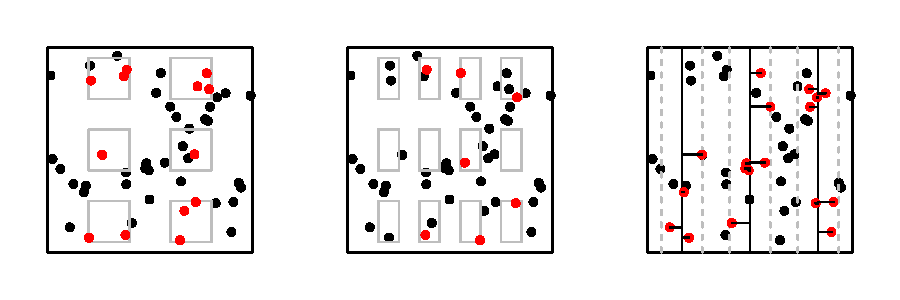
\includegraphics{intro/figs/quadrat-to-ds.pdf}\\
\caption{An example of the performance of quadrat sampling (left), strip transect sampling (middle), and distance sampling (right). Dots indicate individuals, red dots are those in the sample, black those missed. In the first two cases, the grey boxes represent the sampling units. Note that there are many observations just outside of the boxes, which cannot be recorded by survey staff. In the distance sampling case, the solid vertical lines represent the transects and the dashed line gives the effective strip width. Distances are shown by the solid horizontal lines.}
\label{quad-to-ds}
\end{figure}

To make the task of counting the objects within the quadrat easier, one could modify the square design to be a long strip, so that the observer could walk down the centreline of the strip, observing those objects within the strip. Mathematically, if we let the each strip be of width $2w$ and the total length of all strips be $L$, and $n$ objects are observed we have an estimator of the density, $D$:
\begin{equation}
\hat{D}=\frac{n}{2wL}.
\label{ds-simpleD}
\end{equation}
The problem with this approach is that there may well be many objects just outside of the quadrat. Clearly this is a waste of survey effort. It would be preferable to include as many observations as possible and leverage the maximum amount of data we can collect to assess the abundance of the population.

Distance sampling is based on this principle, that if the objects of interest are there then their presence should be recorded. Instead of using fixed-area sampling units, distance sampling requires that only centrelines are specified. The observers should walk (or swim, ride, drive etc) down these observing objects as they go; the distances ($x_i$) to these objects are recorded. Once the survey is complete, the distances are used to estimated the effective area that was sampled. Figure \ref{quad-to-ds} shows the evolution from quadrat to strip to distance sampling.

In equation \ref{ds-simpleD} one can think of replacing $w$ with an estimate of $\mu$, the \textit{effective strip (half-)width}. Further explanation of $\mu$ is given in section SECTIONNUMBER!!! Mathematically, we then have:
\begin{equation}
\hat{D}=\frac{n}{2\hat{\mu}L}.
\label{ds-D}
\end{equation}
We could also consider that a certain proportion ($\hat{P}_a$, the probability of detection) of the objects in a fixed-area ($2wL$) were sampled, so the above can also be expressed as:
\begin{equation*}
\hat{D}=\frac{n}{2wL\hat{P}_a}.
\end{equation*}
Here $w$ is the point after which observations are discarded and is referred to as the \textit{truncation distance}. Truncation is used to discard outliers that make the estimation process tricky. From these two expressions we can see that the relationship between $P_a$ and $\mu$ is $P_a=\mu/w$, these quantities will be investigated further below.

A typical example of line transect data is shown in figure \ref{ds-lt-example}. The figure shows a histogram of perpendicular distances. Note how, as distance increases the number of detections decreases. This characteristic will be exploited later.

% example of line transect data
\begin{figure}
\centering
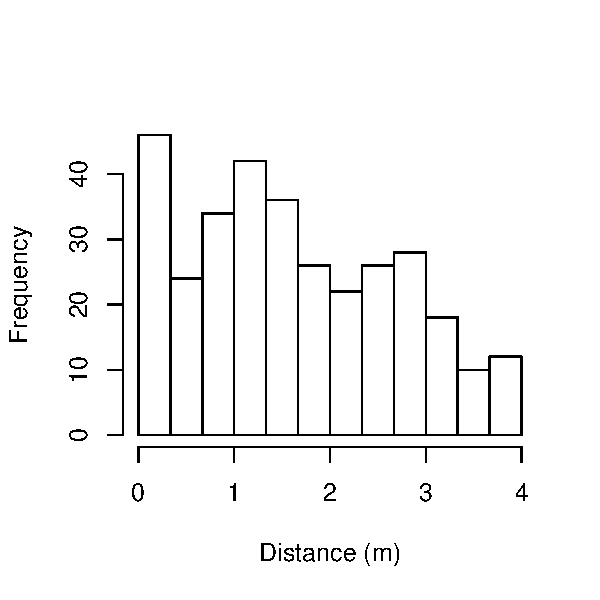
\includegraphics{intro/figs/ds-golftee.pdf}\\
\caption{A histogram of line transect data. In this case from an experiment conducted at the University of St Andrews. 760 golf tees were randomly distributed over a $1680$m$^2$ area, then observed in 11 transects by 8 independent surveys. Further detail may be found in \cite{ADS} p. 140 and \cite{yellowbook}.}
\label{ds-lt-example}
\end{figure}

\subsection{Point transects}
First note that line transects are not the only way of collecting data to put into a distance sampling analysis; point transects may also be used. When using point transects the observer stands at one of a series of points ($m$, say) and observes the objects surrounding him/her. Again, distances to the objects ($r_i$) are recorded. An effective radius ($\rho$) is then calculated, analogously to $\mu$ and then object density can be written as:
\begin{equation}
\hat{D}=\frac{n}{m \pi \hat{\rho}^2}=\frac{n}{m\pi w^2\hat{P}_a}.
\end{equation}
again, the relation between these quantities will be explained below.

An example of point transect data is given in figure \ref{ds-pt-example}. In contrast to the line transect case, there are very few observations near 0, they increase to a point and then fall off beyond that. Note that as the distance, $r$, from the point increases the area surveyed increases as $r^2$. Rescaling this histogram by the areas corresponding to the centre points of the bars will give a histogram that looks like figure \ref{ds-lt-example}.

% example of point transect data
\begin{figure}
\centering
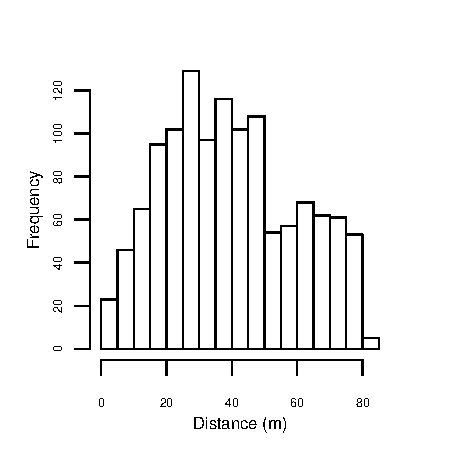
\includegraphics{intro/figs/pt-data-example.pdf}\\
\caption{A histogram of point transect data of Hawaiian amakihi (\textit{Hemignathus virens}) taken from \cite{amakihi}.}
\label{ds-pt-example}
\end{figure}


\subsection{Assumptions}
In order to ensure that estimation is unbiased several assumptions are made. These are summarised below, more information (especially with regard to field procedure) may be found in \cite{IDS}, chapter 2.

\begin{itemize}
	\item The survey must be performed and designed properly and field procedure followed. No amount of analysis can correct for this.
	\item Objects are distributed according to some stochastic process throughout the area of interest.
	\item Lines and points are randomly placed (with respect to the population) and a sample of $n$ objects are detected, measured and recorded.
	\item Objects on the line (or point) are detected with probability 1.
	\item Objects are observed in their initial location, not after movement in response to the observer.
	\item Distances are accurate.
	\item Objects are correctly identified.
\end{itemize}


\subsection{The detection function}
One would expect that the number of animals observed would decrease as the distance of them from the line increased. Correspondingly, one would therefore expect that the probability of seeing an animal would also decrease as a function of distance. This is the relationship captured by the detection function.

The concept of the detection function ($g(x)$) is central to distance sampling. The definition is given as (\cite{IDS}, p. 10):
\begin{equation*}
g(x)=\prob{\text{object detected} | \text{object was at distance } x}.
\end{equation*}
The assumption being that objects' detectability is a function of their distance from the observer. Before talking about models for $g(x)$, we look at the desirable properties.

First off, as stated in the assumptions above, objects on the line are detected with certainty, so $g(0)=1$. Second, it is preferable to have a model where detection is almost certain near zero distance, i.e. that the function has a ``shoulder''. This is physically realistic since the observer should see most things close to him/her. Third, it is also desirable that the model for the detection function is robust, in the sense that it is flexible and can take many plausible shapes. Finally, it is desirable to have a model that is efficient, in the sense that estimates have a relatively small variance, however this is only of use when the other criteria are met.

We now must specify the functional form for $g$. \cite{buckland92} gives a ``key function plus adjustment terms'' formulation for the detection function. The idea is that the key function is used as a starting point for the basic shape of the detection function. The adjustment terms consist of a series expansion that improve the fit of the model. The adjustment terms may not be necessary, in which case they may be left out of the model. The key function is usually selected as one of a uniform, half-Normal or hazard-rate (\cite{buckland85}) function. The adjustment terms are typically either even simple polynomials, Hermite polynomials or cosine functions. Further information can be found in \cite{IDS} p.47. Figure \ref{ds-detfct-examples} shows some possible detection functions.

% Possible detection functions
\begin{figure}
\centering
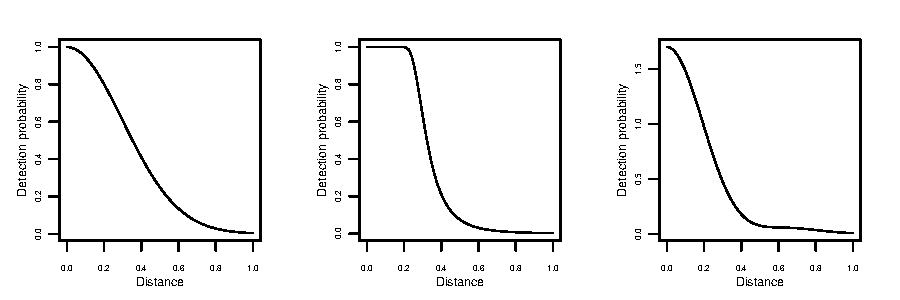
\includegraphics{intro/figs/detfct-examples.pdf}\\
\caption{Three possible detection functions. The first is a half-Normal distribution, the second a hazard-rate function and the third the same half-Normal as the first but with a cosine adjustment term. Notice that the hazard-rate has a controllable ``shoulder''.}
\label{ds-detfct-examples}
\end{figure}

This formulation leads to a class of highly flexible models and a normal analysis may consist of running models made up of various combinations of key functions and adjustment terms. Model selection is usually performed using AIC.






\subsection{From $g(x)$ to $D$}

Equation \ref{ds-D}, above shows that in order to estimate the density of the population in question, we must estimate $\mu$, the effective strip width. To do this we must use the detection function.


\subsubsection{Line transects} 
As mentioned above, $\mu$ is defined to be the distance from the lines for which as many objects are detected beyond $\mu$ as are missed within $\mu$ (\cite{eenviron}). Looking at figure \ref{ds-mu-explanation}, the shaded area above the curve (the detection function) represents those objects that were there up to a distance of $\mu$ from the line, but were missed by the observer. The shaded area below the curve represents those objects that were observed beyond a distance $\mu$. By moving $\mu$ to the left or to the right, it is possible to find a point at which the two shaded areas are of equal size. This fulfils the criterion for $\mu$.

% explanation of mu
\begin{figure}
\centering
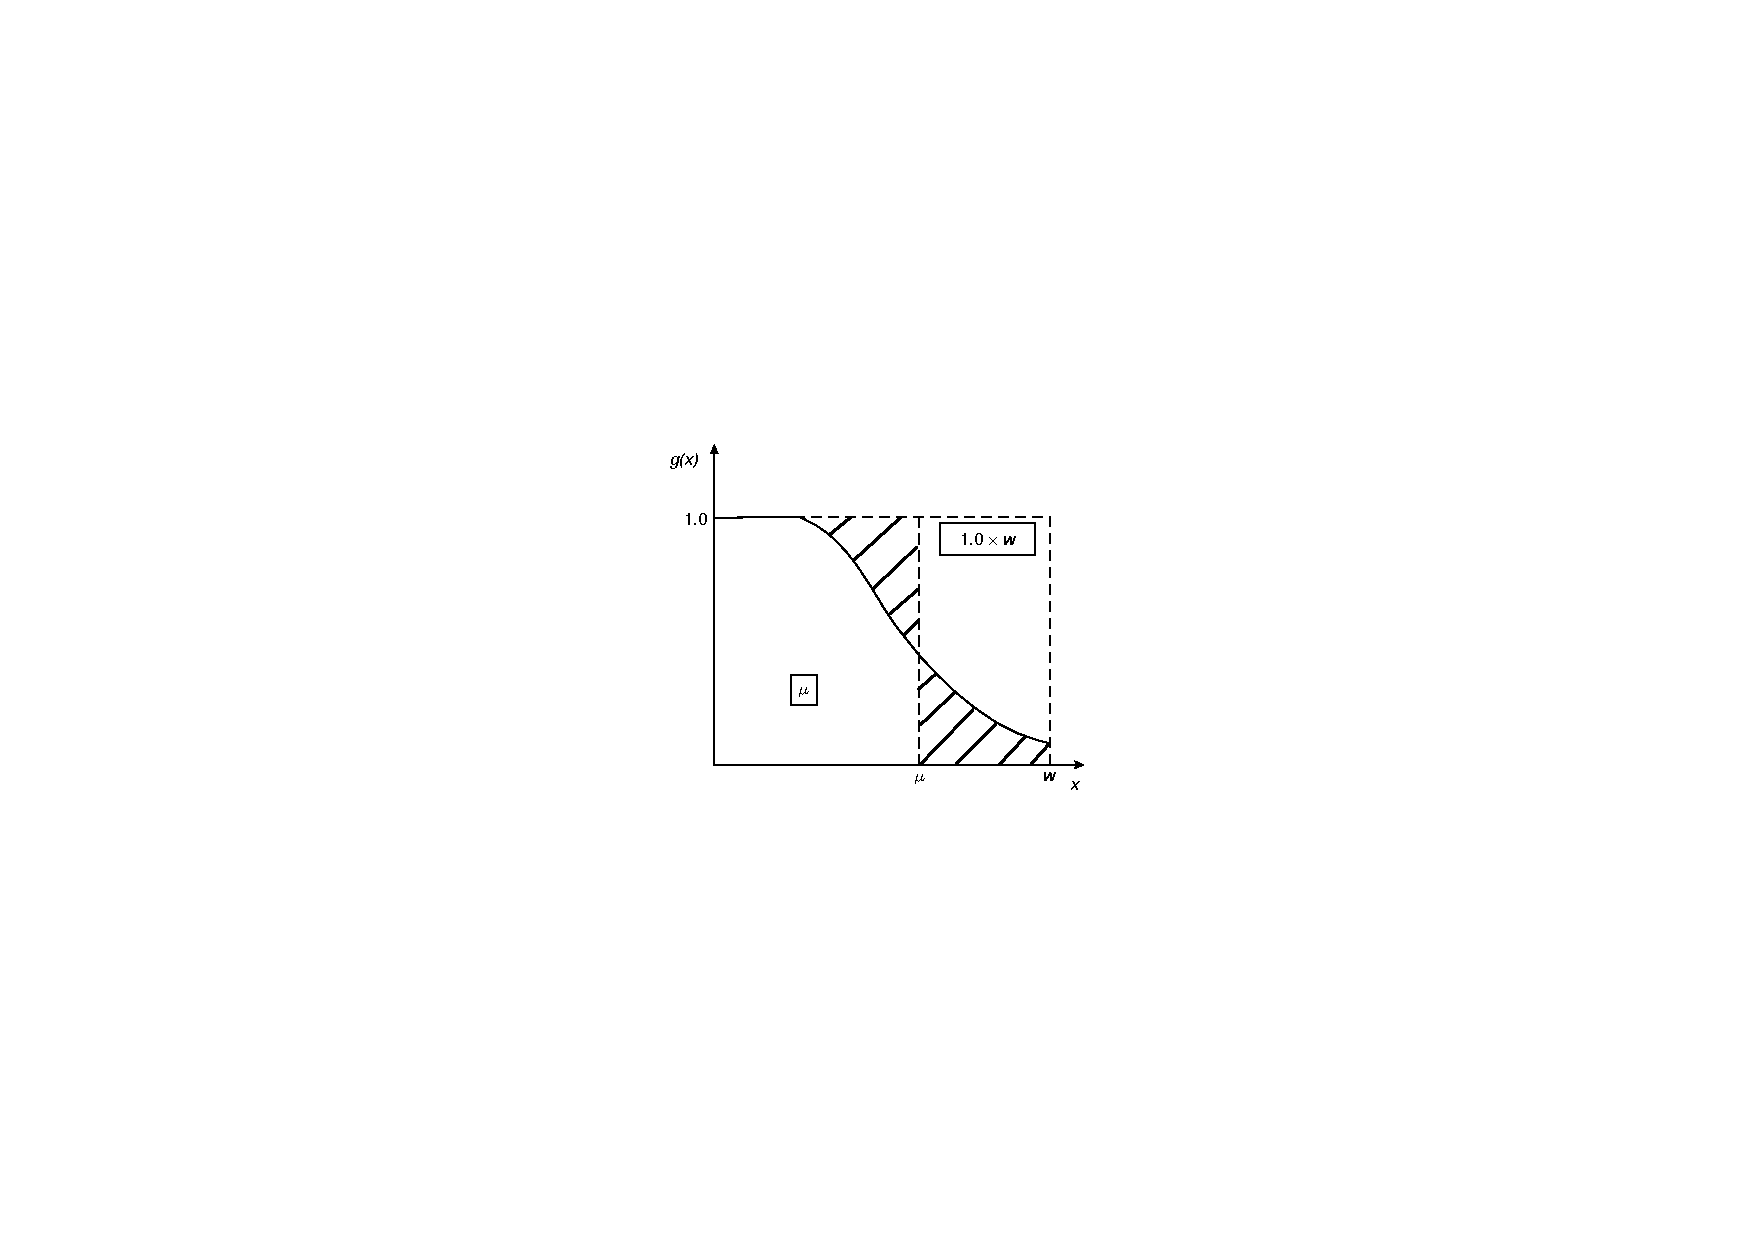
\includegraphics{intro/figs/muexplanation.pdf}\\
\caption{REDRAW THIS}
\label{ds-mu-explanation}
\end{figure}

Now the question is: how is $\mu$ calculated? Note that the rectangle with side $0$ to $1$ on the $y$ axis and $0$ to $\mu$ on the $x$ axis has area $\mu$ and that this is the same as the area under the detection function. So, $\mu$ is also the distance out to which we observe everything and it is defined as:
\begin{equation}
\mu = \int_0^w g(x) \text{d}x.
\label{ds-lt-mu-def}
\end{equation}
where $w$ is again the truncation distance and ignoring the functional form of $g(x)$. Hence $P_a$ is defined as:
\begin{equation*}
P_a = \frac{\int_0^w g(x) \text{d}x}{w}.
\end{equation*}
Substituting this expression into (\ref{ds-D}), we obtain:
\begin{equation*}
\hat{D}=\frac{n}{2L \int_0^w \hat{g}(x) \text{d}x}.
\end{equation*}
Now let us assume that $g(x)$ has some fixed functional form and that we wish to estimate its parameter(s) (which for now will be referred to as $\bm{\theta}$). This can be done via standard maximum likelihood methods. First we must find a probability density function. Note that the expected number of objects at a distance $x$ from the transect line (including those not observed) is independent of $x$. This then implies that the shape of the density functions is the same as that of the detection function and can therefore be obtained by rescaling (\cite{IDS}, p. 38). So, the pdf of the perpendicular distance data, conditional on the object being observed is then:
\begin{equation}
f(x;\bm{\theta}) = \frac{g(x;\bm{\theta})}{\int_0^w g(x;\bm{\theta}) \text{d}x} = \frac{g(x;\bm{\theta})}{\mu}.
\end{equation}
As an aside, note that by the assumption, above, $g(0;\bm{\theta})=1$, so:
\begin{equation}
f(0;\bm{\theta}) = \frac{g(0;\bm{\theta})}{\int_0^w g(x;\bm{\theta}) \text{d}x} = \frac{1}{\mu}.
\end{equation}
Now we have obtained an expression for the pdf, we can form a likelihood:
\begin{align}
\mathcal{L}(\bm{\theta}; \bm{x}) &= \prod_{i=1}^n f(x_i;\bm{\theta}),\\
&= \prod_{i=1}^n \frac{g(x;\bm{\theta})}{\mu}.
\label{ds-lt-likelihood}
\end{align}
The log of this quantity can then be used as an objective function in an optimisation procedure in order to find the maximum likelihood estimators of the parameters, $\bm{\theta}$.

\subsubsection{Point transects} 

Point transects follow an analogous explanation to line transects. Instead of effective strip width, we look at effective area of detection. 

For line transects, an infinitesimal strip has area $L\text{d}x$ (that is the length of the line, multiplied by an infinitesimal distance perpendicular to the line) and this value is independent of $x$. However, in the point transect case an incremental annulus depends on $r$ (the distance from the point), such an annulus has area $2\pi r \text{d}r$. So, the effective area of detection is therefore defined as:
\begin{equation}
\nu = 2 \pi \int_0^w r g(r) \text{d}r.
\end{equation}
Then, following through the arguments above, we can define the PDF as:
\begin{equation}
f(r) = \frac{r g(r)}{\int_0^w r g(r) \text{d}r},
\end{equation}
and hence: 
\begin{equation}
f(r) = \frac{2 \pi r g(r)}{\nu},
\end{equation}
a more rigorous proof of this is given in \cite{IDS} p. 54.

By analogy to the line transect case the relation between $\nu$ and $P_a$ in the point transect case is
\begin{equation}
P_a=\frac{\nu}{\pi w^2}
\end{equation}
so
\begin{equation}
f(r) = \frac{2 \pi r g(r)}{\pi w^2 P_a}.
\end{equation}
So again, a likelihood can be formed:
\begin{align}
\mathcal{L}(\bm{\theta}; \bm{r}) &= \prod_{i=1}^n f(r_i;\bm{\theta}),\\
&= \prod_{i=1}^n \frac{2 \pi r g(r;\bm{\theta})}{\nu}.
\end{align}
As above, the log of this expression can then be used in an optimisation procedure to find the MLEs of the parameters.


\subsection{Covariates}
One can very easily think of the case in which one or more factors effect the detectability of objects in a survey. A typical example might be sex or size of the object or weather conditions during when the object was observed. When available this information can be very useful in handling heterogeneity in the data (\cite{IDS}, p. 88). Covariates are included in detection function models by using a link function. One (or more) of the parameters of the detection function is considered to be a linear combination of the covariates. Figure \ref{ds-covarex} shows the effect of both continuous and factor covariates on a hazard-rate detection function.

% example covariates and how they effect the detection function
\begin{figure}
\centering
% trim order l b r t
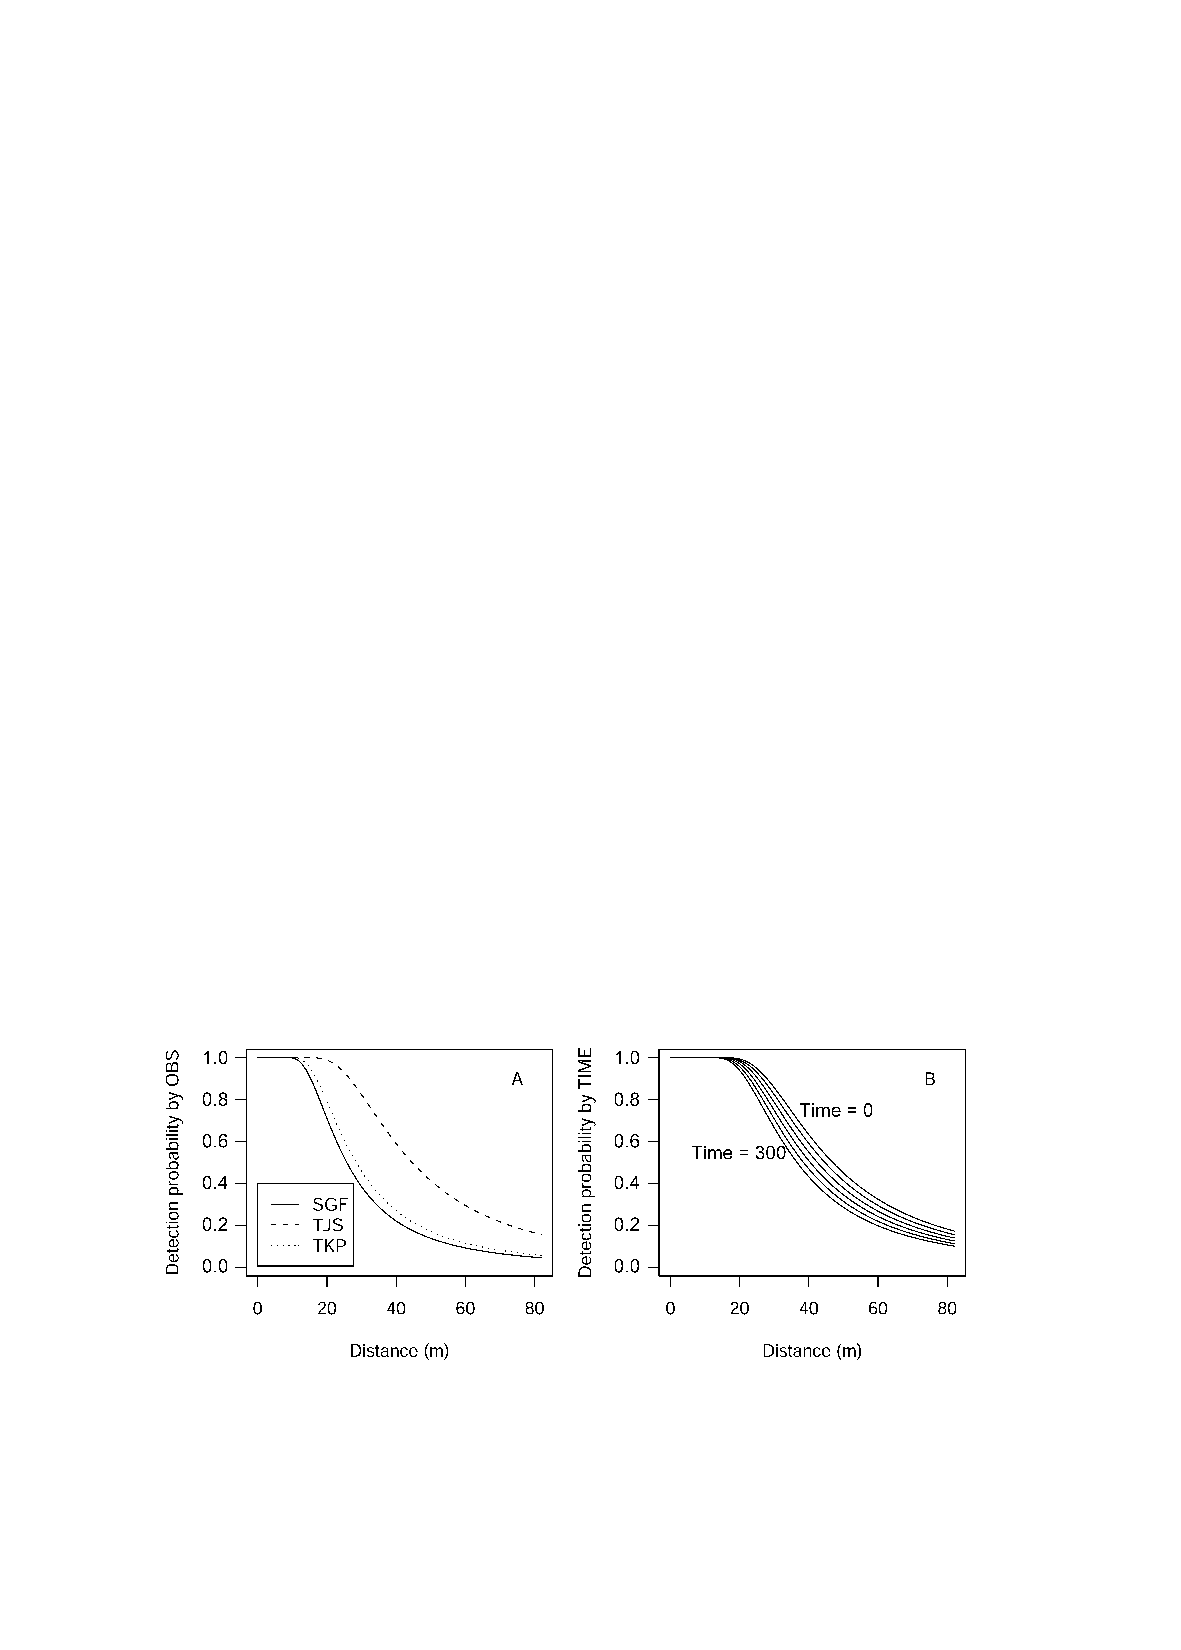
\includegraphics{intro/figs/amakihi-detfct.pdf}\\
\caption{The influence of covariates on the detection function (taken from \cite{amakihi}). The detection functions are for Hawaiian amakihi (\textit{Hemignathus virens}). The left panel shows the effect of a factor covariate (observer), while the right shows the effect of a continuous covariate (time). In each case the other covariate is held constant (time at $0900$ and observer as ``TJS'') while the other is varied.}
\label{ds-covarex}
\end{figure}


Considering a detection function modelled by a half-Normal, we can write that:
\begin{equation}
g(x; \sigma) = \exp\Big(\frac{-x^2}{2\sigma^2}\Big)
\end{equation}
now, say that two covariates have been collected, $z_{i,\text{sex}}$ and $z_{i,\text{Beau}}$ indicating the sex of the animal and the Beaufort sea state when the animal was observed. Also recorded are the distances $x_i$. The covariates can be included in the analysis by considering $\sigma$ as a linear combination of these covariates, so we can either consider their to be one $\sigma$ per unique covariate combination:
\begin{equation}
\sigma_i = \exp( \beta_0 + \beta_1 z_{i,\text{sex}} + \beta_2 z_{i,\text{Beau}}),
\end{equation}
or that $\sigma$ is a function of the covariates and corresponding parameters:
\begin{equation}
\sigma(z_{i,\text{sex}}, z_{i,\text{Beau}}; \beta_1, \beta_2) = exp(\beta_0 + \beta_1 z_{i,\text{sex}} + \beta_2 z_{i,\text{Beau}})).
\end{equation}
Of course, these expressions are equivalent, the latter will be used throughout for clarity. We are now interested in obtaining estimates of $(\beta_0, \beta_1, \beta_2)$.

More generally the notation for the detection function is $g(x ; \sigma(\bm{z}; \bm{\beta}))$ where $\bm{z}$ is the $K$-vector of the covariates $z_1, \dots, z_K$ related to the observation $x$. The complete set of covariates for all observations is stored in $Z$, an $n \cross K$ matrix. The scale function is referred to as $\sigma(\bm{z}; \bm{\beta})$ to clarify when covariates are used.

This covariate formulation can be thought of as a generalisation of the non-covariate model, the latter simply being the case where there is only an intercept term. This is equivalent to log-transforming the scale parameter.

This formulation fits nicely into the likelihood expressions above, the evaluations of the detection function are as above, but the calculation of $\mu$ (and therefore $P_a$) changes. It is now the case that we think of both of these quantities as functions of the covariates, as we did for $\sigma$.

The effective strip width, $\mu$ is now expressed as:
\begin{equation}
\mu(\bm{z}_i) = \int_0^w g(x ; \sigma(\bm{z}; \bm{\beta})) \text{d}x,
\end{equation}
and following from the relation between $\mu$ and $P_a$, above we define:
\begin{equation}
P_a(\bm{z}_i) = \frac{\int_0^w g(x ; \sigma(\bm{z}; \bm{\beta})) \text{d}x}{w}.
\end{equation}
Similarly for point transects, the probability of detection and $\nu$ are given as:
\begin{equation}
P_a(\bm{z}_i) =\frac{2}{w^2}\int_0^w r g(r; \sigma(\bm{z}; \bm{\beta})) \text{d}r, \qquad \nu(\bm{z}_i) = \int_0^w r g(r; \sigma(\bm{z}; \bm{\beta})) \text{d}r
\end{equation}

With this formulation, abundance can be estimated by a Horvitz-Thomspon-like estimator (\cite{thompson}, pp. 53-56, \cite{ADS}, p.23):
\begin{equation}
\hat{N} = \sum_{i=1}^n \frac{1}{P_a(\bm{z}_i)}.
\end{equation}

\subsection{Other considerations}
\subsubsection{Line and point placement}
The placement of the lines and points above is said to be ``random'', in practise randomly placing and orientating lines can be expensive and time-consuming (in particular in shipboard surveys where one wishes to minimise off-effort time). The solution to this is simply randomly placing and orientating a grid of lines or points. For shipboard surveys ``zigzag'' designs can be used to minimise off-effort time (\cite{strindberg04}). It is also important to ensure that transects to not run parallel to geographical features to avoid bias. For example using roads as transects (as was done in the US breeding birds survey) leads to bias since animals may be compelled to move away from the road and toward neighbouring hedgerows (\cite{IDS}, p. 18).

\subsubsection{Clusters}
If animals are observed in clusters (for example pods for whales or packs for wolves) then it might be more convenient to estimate the abundance of clusters and use them as the fundamental unit to estimate. The cluster size can also be estimated and the abundance of clusters ``multiplied up'' to give the overall abundance (\cite{IDS}, p. 13). It is assumed throughout that the analysis is dealing with individuals rather than clusters.



\subsection{Summary}
Distance sampling is unlike most methods in statistics, in that the quantity which we wish to find, abundance, is not given explicitly in the likelihood we wish to optimise. Instead we wish to find the parameters for the detection function, to then estimate of $\mu$, in order to estimate density (and hence the abundance). Contrasting this with capture-recapture, where the abundance is obtained directly from finding the MLE of the parameters, it seems rather complex and esoteric. 

Distance sampling benefits from a relatively simple field procedure, a wealth of literature and easy to use software for analysis. Distance sampling has also been adapted for many different scenarios, including analysing data which was not initially part of a survey (incidental data).

Non-covariate distance sampling, as described above, is commonly referred to as CDS (conventional distance sampling) and covariate distance sampling as MCDS (multiple covariate distance sampling. Other variants exist, for example mark-recapture distance sampling (MRDS, see \cite{mrdspaper}) and spatial distance sampling models (see chapter 4 of \cite{ADS}.

\subsection{Monotonicity}
One potential pitfall of both CDS and MCDS is that  it is possible to formulate models which are not physically realistic. In particular it is possible to create models which are non-monotonic functions of distance. Data with a mode away from zero distance may occur when there has been heaping, when objects move prior to observation or just by chance; fitting models to such ``bumps'' can cause bias in abundance estimates (\cite{IDS}, p. 132). To get around this problem \cite{distance-software} constrains the detection function to be monotonic. This is done by taking 10 equally spaced distances from $0$ to $w$ and checking that when the detection function is evaluated at each of these points they are less than the last (mathematically, $g(x_i)\geq g(x_{i+1})$ for distances $x_1 \dots x_10$ where $x_1=0$). This is referred to as \textit{strong monotonicity}. Alternatively users may opt for \textit{weak monotonicity} where each point is checked only against the value of $g$ at the origin (mathematically, $g(0)\geq g(x_i)$) or, to turn this off completely.

Constraining the likelihood is appealing here, however it is obviously always preferable to perform unconstrained optimisation if possible. Using a class of functions to model the detection function which were both flexible and did not exhibit the undesirable property of non-monotonicity could offer a more physically realistic and convincing alternative to the conventional way of performing distance analyses.

Finally, note that although constraining the shape of the detection function is possible, it does not necessarily lead to monotonic detection functions. Figure \ref{humpback-nonmono} shows a detection function fitted to humpback whale data (taken from \cite{williams}). Here a half-Normal key function with a cosine adjustment term was fitted to the data and, although constraints were used, the function is still monotonic.

% example of non-monotonic detection function - humpback
\begin{figure}
\centering
% trim order l b r t
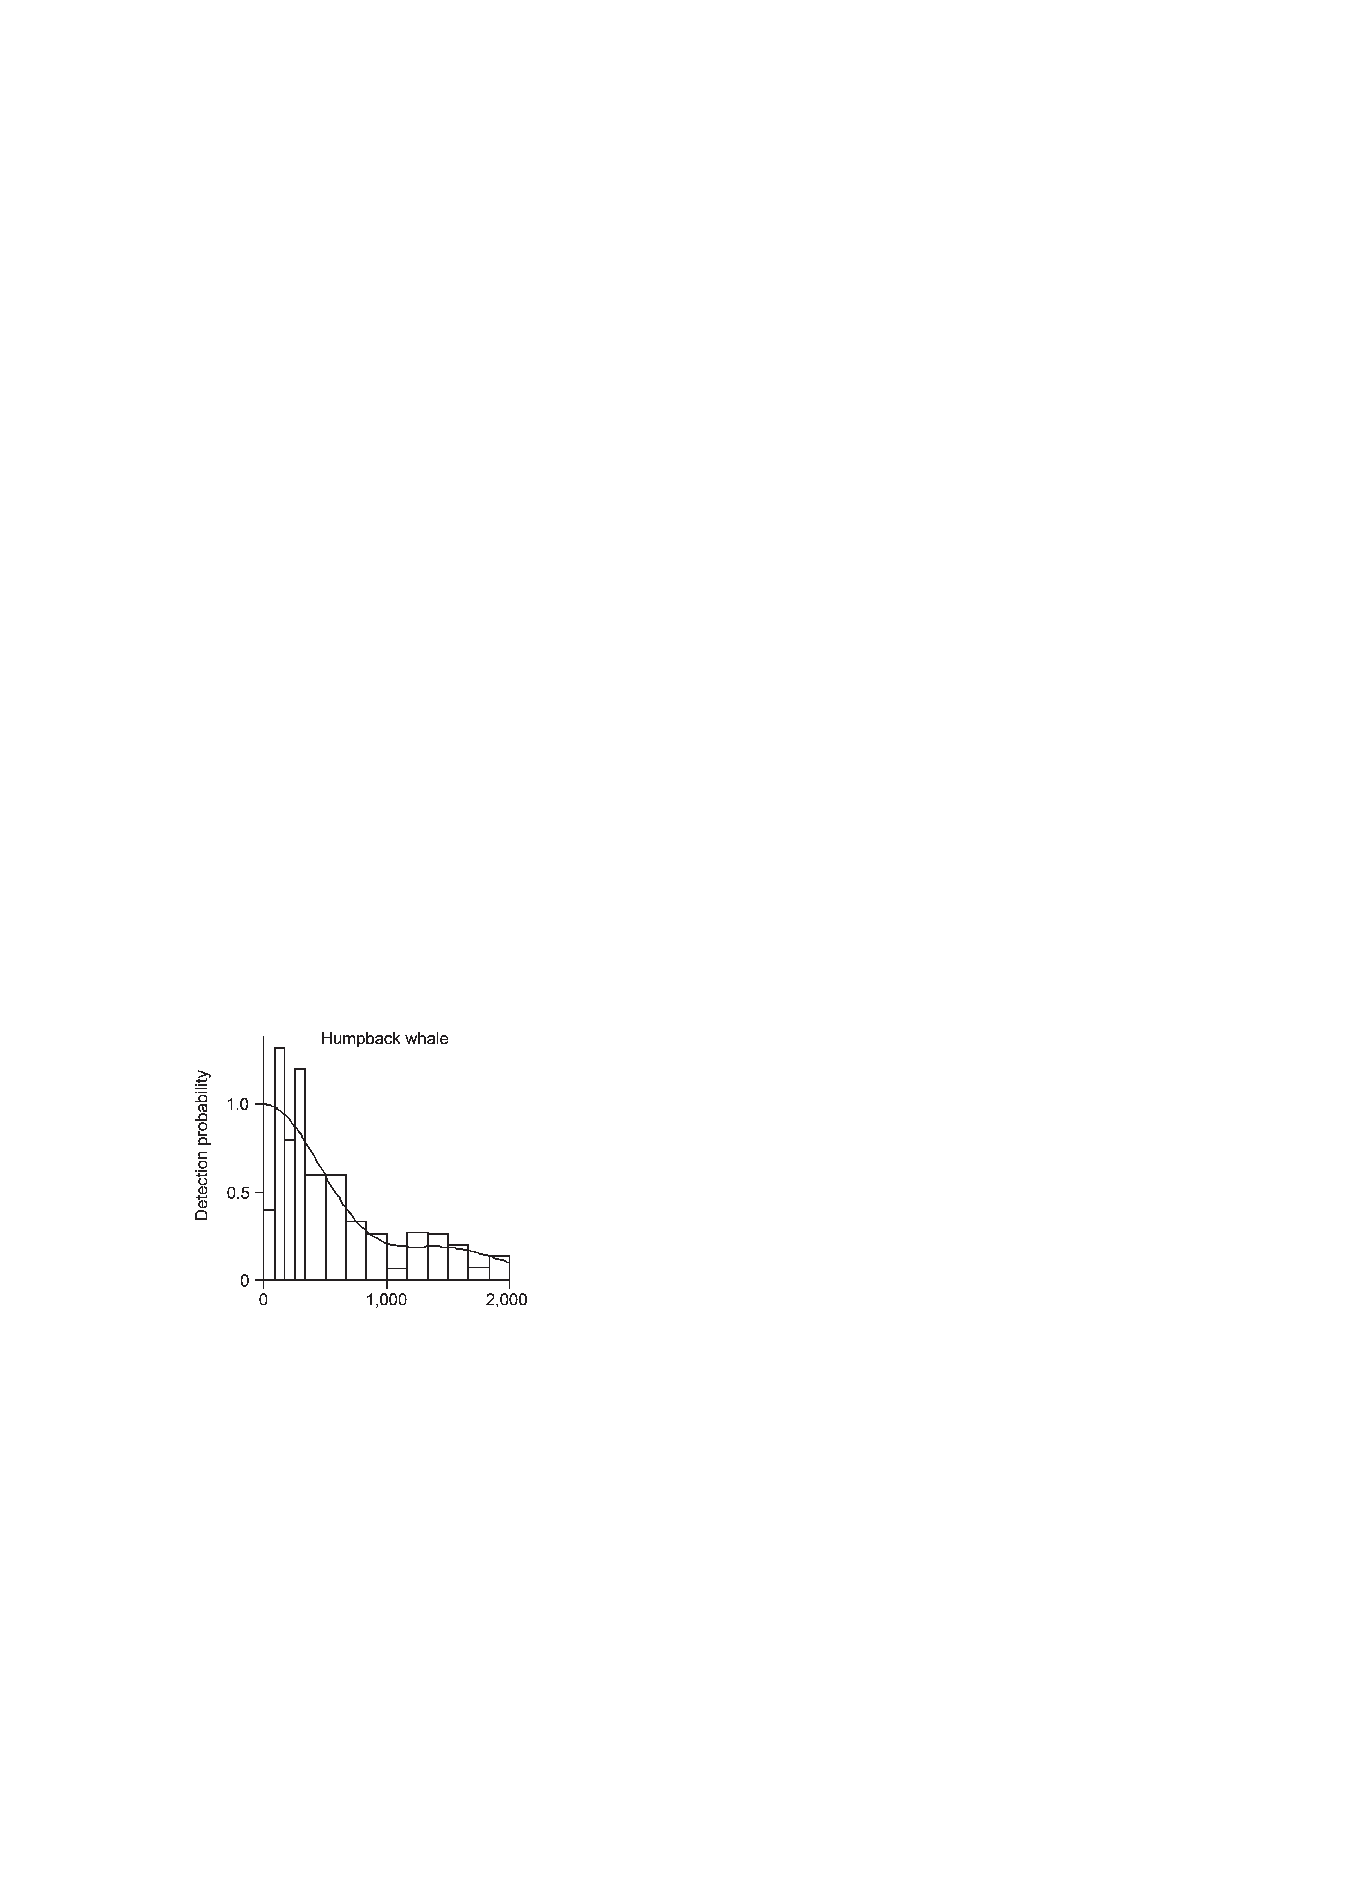
\includegraphics{intro/figs/humpback-nonmono.pdf}\\
\caption{Humpback whale data from \cite{williams} with a half-Normal key function with a cosine adjustment overlaid. Constraints have failed to ensure that the function is monotonic. Figure taken from \cite{williams}.}
\label{humpback-nonmono}
\end{figure}




\subsection{Mixture models}
Recently developments, particularly in mark-recapture (\cite{pledger2000}, \cite{dorazio03}, \cite{pledger2005} and \cite{morgan08}) have shown that mixture models can be an extremely useful and flexible method of modelling heterogeneity in biological populations.

Covariates provide some information on those factors which may effect the detectability of individuals, modelling some of the heterogeneity in the detection process. Adjustment terms attempt to perform a similar task (though in an admittedly blunter fashion) by smoothing the function of distance in a semi-parametric way. A combination of the two approaches is possible although some have philosophical opposition to it (Jeff Laake, personal communication). Aside from this, the practical issue of monotonicity is problematic; one would like to both handle heterogeneity with both the data at hand (in the form of covariates) whilst also ``smoothing away'' residual effects of unobserved states in the population.

Mixture models provide models that can handle these situations in a parsimonious way. Consider the following example: it is known that for a particular species the female is much easier to observe than the male (for example, in a song bird the female might be more vocal) however the two sexes are indistinguishable to an observer so no covariate can be recorded. The two sexes form two distinct classes in the sample but are unobserved. Since the female is easier to observe than the male, the two classes will have different detection functions. A distance sampling analysis using adjustment terms will attempt to model the average of the two detection functions. Instead one could use a mixture model for the detection function. A weighted combination of two functions could then be used to describe the two different classes and their proportions in the sample. 

The logical extension of this approach is to include covariates in the mixture model too. Say, for example, that it is possible to identify the age of the animal but not the sex, the age can be included as a covariate and the ages classes can again be modelling using the mixture. Note that there is no classification going on here: there is no decision over whether observations are, say, male or female. Rather the proportions of each are being estimated along with the parameters of their respective detection functions.

% example of composite detection function
\begin{figure}
\centering
% trim order l b r t
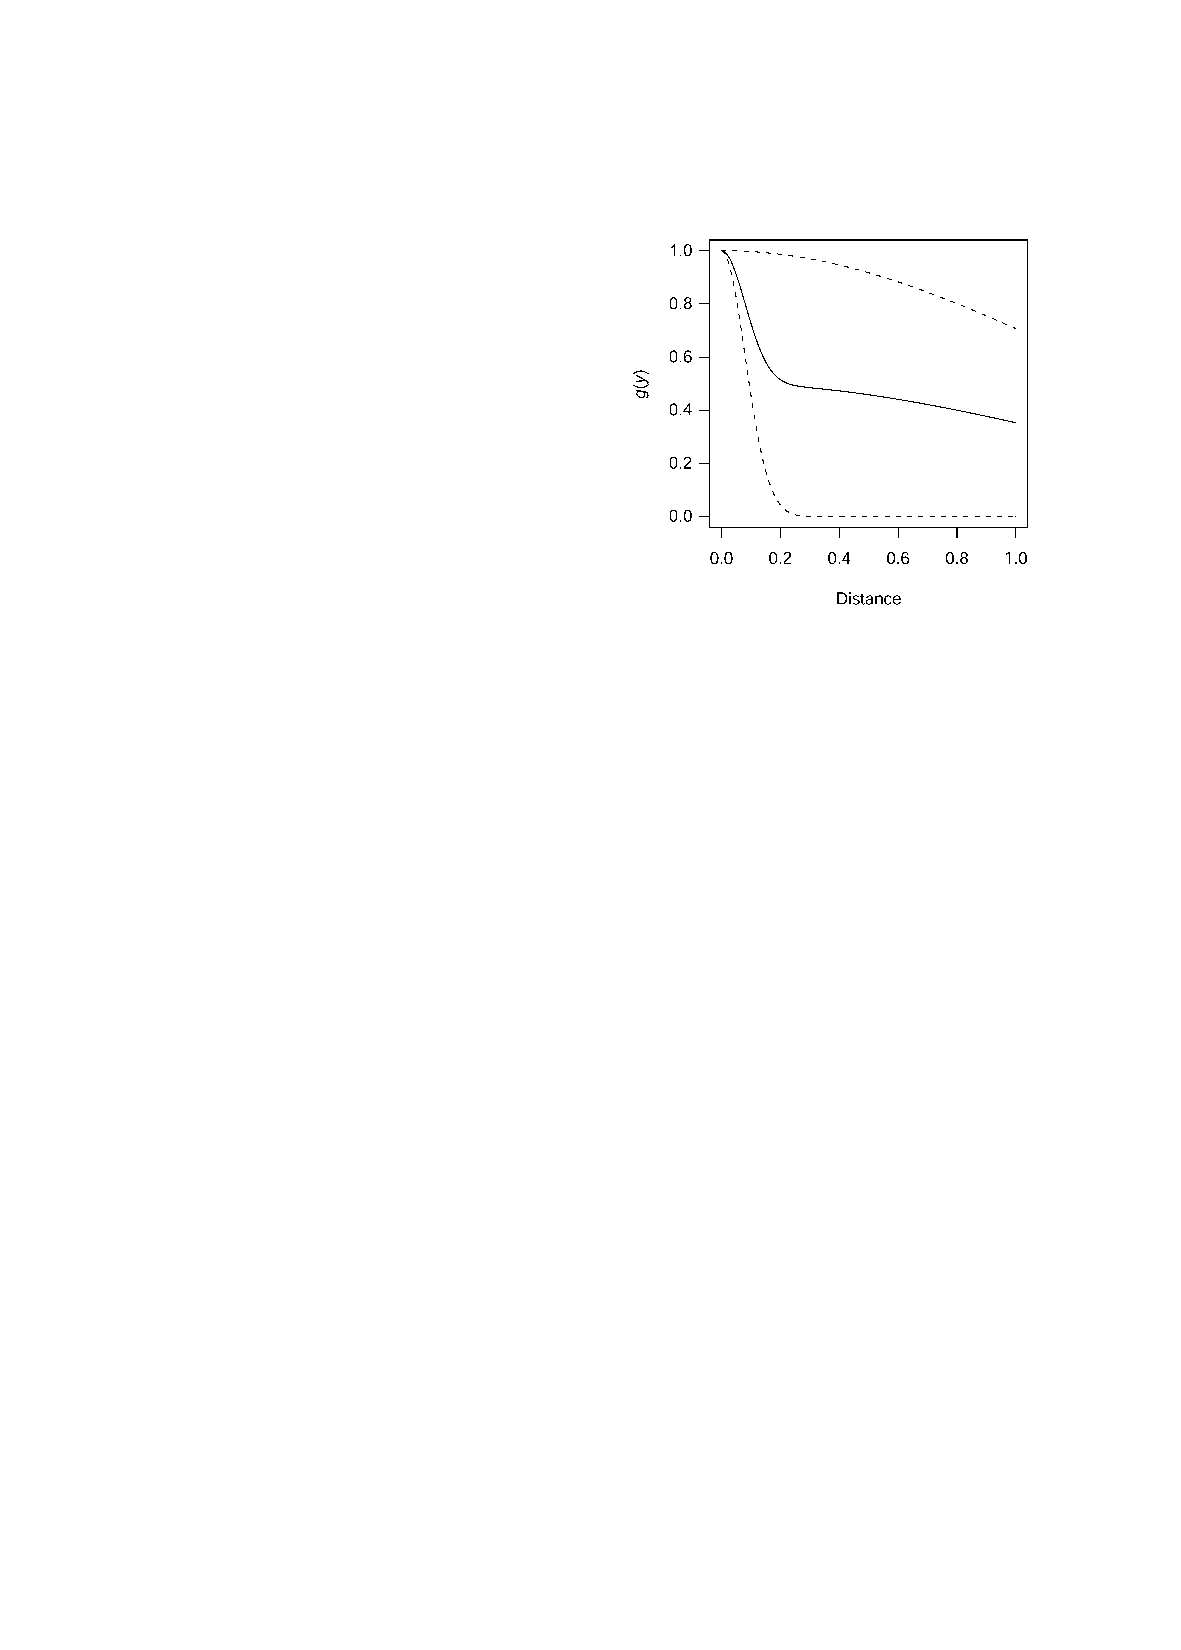
\includegraphics{intro/figs/malefemale-detfct.pdf}\\
\caption{A detection function (solid line) composed of two other detection functions (dashed lines) representing two parts of a population. The spike could represent less vocal males and the detection function with the wider shoulder could represent the more vocal (and hence more easily observable) females (for example).Taken from \cite{amakihi}.}
\label{ds-malefemale-detfct}
\end{figure}

Figure \ref{ds-malefemale-detfct} shows the effect that might be seen when one subsection of the population (say females) are more detectable than another (males). Where the information on sex is available, a covariate analysis should be able to separate these two populations. If it is not, a CDS analysis will yield unsatisfactory results.

If only monotonic functions are used in the mixture then a monotonic detection function will result as any sum of monotonic functions is, itself, monotonic. This avoids the problems of constrained optimisation inherent in the ``key function plus adjustment terms'' formulation currently used.

Finally, the approach is also interesting for its own sake. There is no current literature on the use of mixture models as detection functions for distance sampling. Many detection function forms have been proposed (for example, \cite{buckland92} and  \cite{gammadetfct}), each having their own merits and pitfalls.





